%!TEX root = Thesis.tex

\chapter{Constraints Unification for Configurable Layout Manipulation}\label{chap:CUCLM}
  \section{Introduction}\label{sec:CUCLMIntro}

    Typically, in order to prevent a design from mismatching and losing symmetry after placement and routing, a number of conditions instructed by designer should be followed. Many applications refer to their self-defined rules by particular semantics. In addition to the design purposes, the technology process rules from the foundry is of equal importance to an analog layout design. Traditionally, it is time-consuming analog layout design flow due to iterative design-rule-check and re-design operation. Hence, it is important to integrated a design-rule interactive-check into a constraint driven model for automatic analog design. 

    The OpenAccess constraint model standardizes different kinds of design guidelines, process rules and electrical constraints in a general specification for all users. OpenAccess constraint model provides a general constraint format for tool developers, foundries and analog designers to establish distinctive constraints. Moreover, besides the built-in semantics of constraints, an extensible mechanism of OpenAccess constraint can offer the flexibility for particular specifications. Thus, the analog designs can facilitate to define constraints with such extension ability. In addition, OpenAccess also supports {\bf constraint group} format in order to gather constraints in the same type as a group. For example, the process rules constraints are gathered as the {\bf foundry} constraint group, and the design objective constraints consist of the {\bf user-defined} constraint group. Also, a constraint group can be a member of another constraint group recursively. As a result, a series of constraint groups hierarchically constructs the top-down constraint topology in database. 

    \begin{figure}[t]
      \centering
      \centerline{
        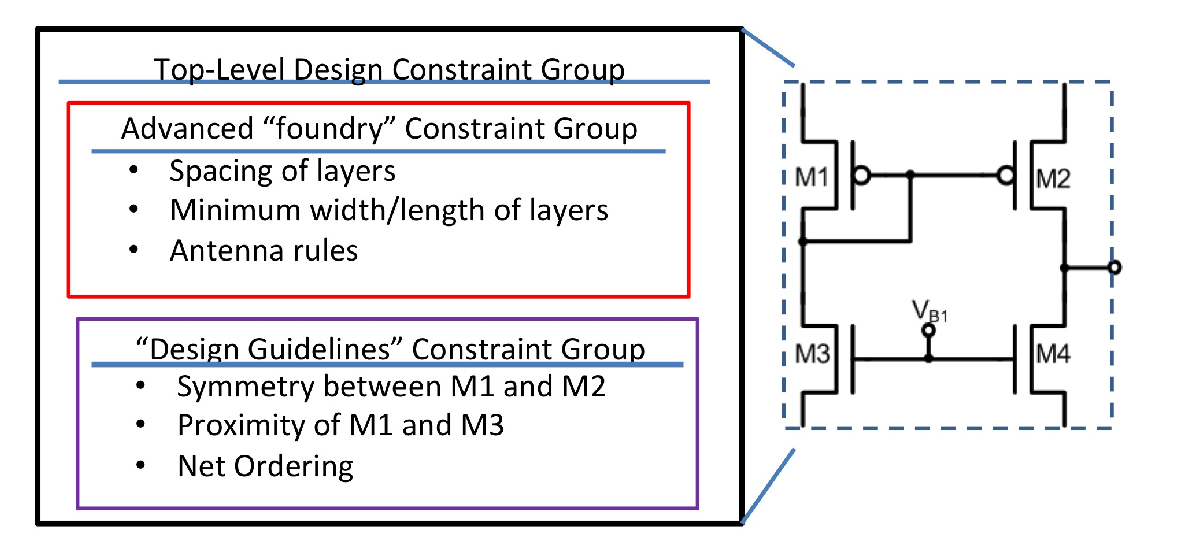
\includegraphics[width=0.7\textwidth]{Fig/Chapter3/CGSample0.eps}
      }
      \caption{A typical design which is accompanied with constraint groups.}
      \label{fig:CGGrouping}
    \end{figure}    
    
    %Fig.~\ref{fig:CG} shows the hierarchical relationship of OA constraint. 
    A design library consists of reference technology library and the top-level design. The top-level design is formed with multiple level reference designs. A collection of constraint group owned by the top-level design includes constraints from the technology library, the user-defined constraint group, the built-in constraint group and the particular constraints for this design. Similarly, the reference design in the sub level also accompanies the constraints in the same structure as its parent. We give an obvious case in Fig.~\ref{fig:CGGrouping}. A current mirror style design and its constraint group are shown. This constraint group is composed of two different kind of constraint groups: the {\bf foundry} and {\bf design guidelines} constraint groups. The basic design rules of the specific technology forms the {\bf foundry} constraint group, such as different technology nodes on  65nm or 40nm. The {\bf design guidelines} constraint group represents the constraints which are strictly owned by the design, such as symmetrical group, matching property and the net order information.

  \section{Constraint Generation and Unification}\label{sec:ConGenUni}

    According to Fig.~\ref{fig:LayoutFlow}, the constraint driven routing methodology attempts to generate the layout-oriented constraint groups in post-placement layout. In this section, we provide a flow to generate constraint group for routing purpose from required technology process rules, design guidelines and layout topology. 
  
    The detail flow of constraint group generation is shown in Fig.~\ref{fig:LayoutCGGen}. From the beginning of our constraint group generation flow, we feed an analog layout design with cell location and connectivity informations into our constraint group generator. Our constraint group generation flow has three stages: Process rule constraint group generation, Pre-defined design guidelines constraint group generation and the Layout constraint extractor. The first stage is necessary, and the second is prior to the third one. In case there is no any constraints being applied in the second stage, this constraint generator tends to extract the constraint from existing layout. In other words, we value the designers' expertise in order to guarantee that the constraint driven routing methodology honors the routing priority as designers' expectation. Here we express the three steps of constraint generation in the following subsections. 
    
    \begin{figure}[t]
      \centering
        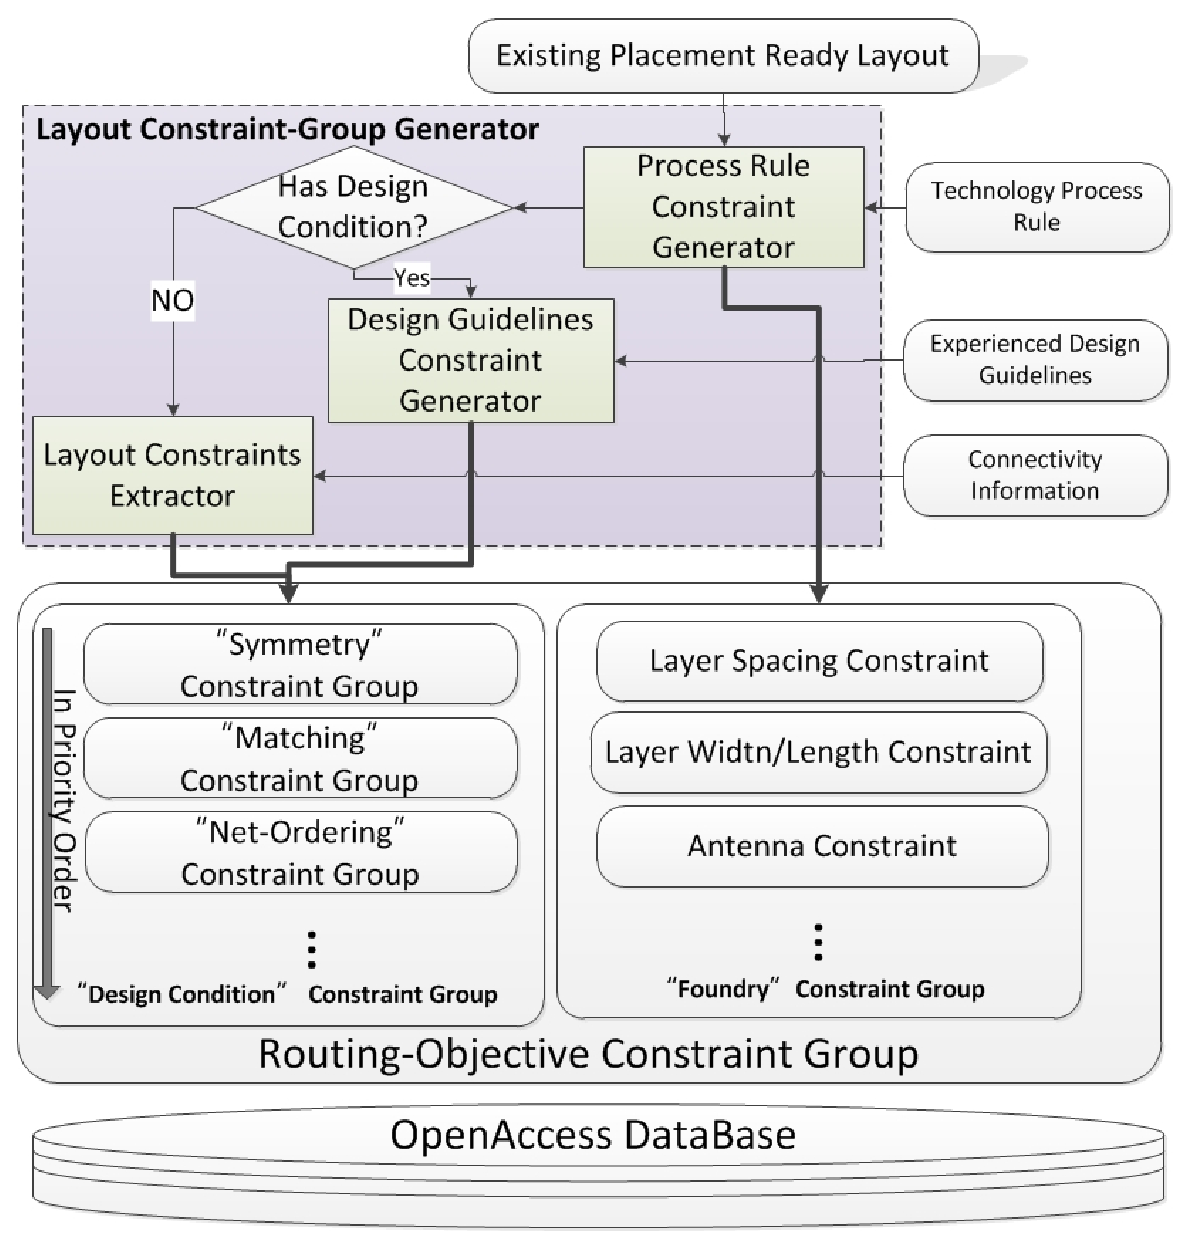
\includegraphics[width=0.5\textwidth]{Fig/Chapter3/LayoutConGen.eps}
        \caption{Layout-oriented constraint generation flow.}
        \label{fig:LayoutCGGen}
    \end{figure}

    \subsection{Process Rules Constraint Group Generation}\label{sec:RCG}
    
      The ``foundry'' constraint group is automatically stored in the technology database under OpenAccess platform. Thus, applications developed on OpenAccess can access the foundry process rule directly before post-layout verification. In other words, the exact process rule can be considered during the placement and routing stage. Traditionally, works implement P\&R methodologies with abstract design ruls because it is complex and time-consuming to import the whole design rule of the target technology as constraints. Other than applying such abstract constraints, the mechanism of built-in constraint groups can check out the exact design rules at runtime stage. It indeed raises the efficiency with respect to fewer redesign cost. Most of the constraints for technology purpose are layer-related. Table~\ref{tableFoundryCon} expresses a group of layer constraints refering to a specific technology. However, according to rule complexity of advanced technologies, the built-in constraint group is inadequate for the new generation technology. 
    
      \begin{table}[ht]
        \centering
        \caption{Basic Foundry constraints}\label{tableFoundryCon}
        \begin{scriptsize}
          \begin{tabular}[t]{|l|l|}
            \hline
            Constraint Type & Value \\
            \hline
            minSpace  & ``METAL2'',0.16 \\
            \hline
            minEnclosure  & ``METAL2'',``VIA2'',0.01  \\
            \hline
            minEndofLineSpacing & ``METAL2'',0.1,0.1,0.42 \\
            \hline
          \end{tabular}
        \end{scriptsize}
      \end{table}
    
    
      \begin{figure}[t]
        \centering
        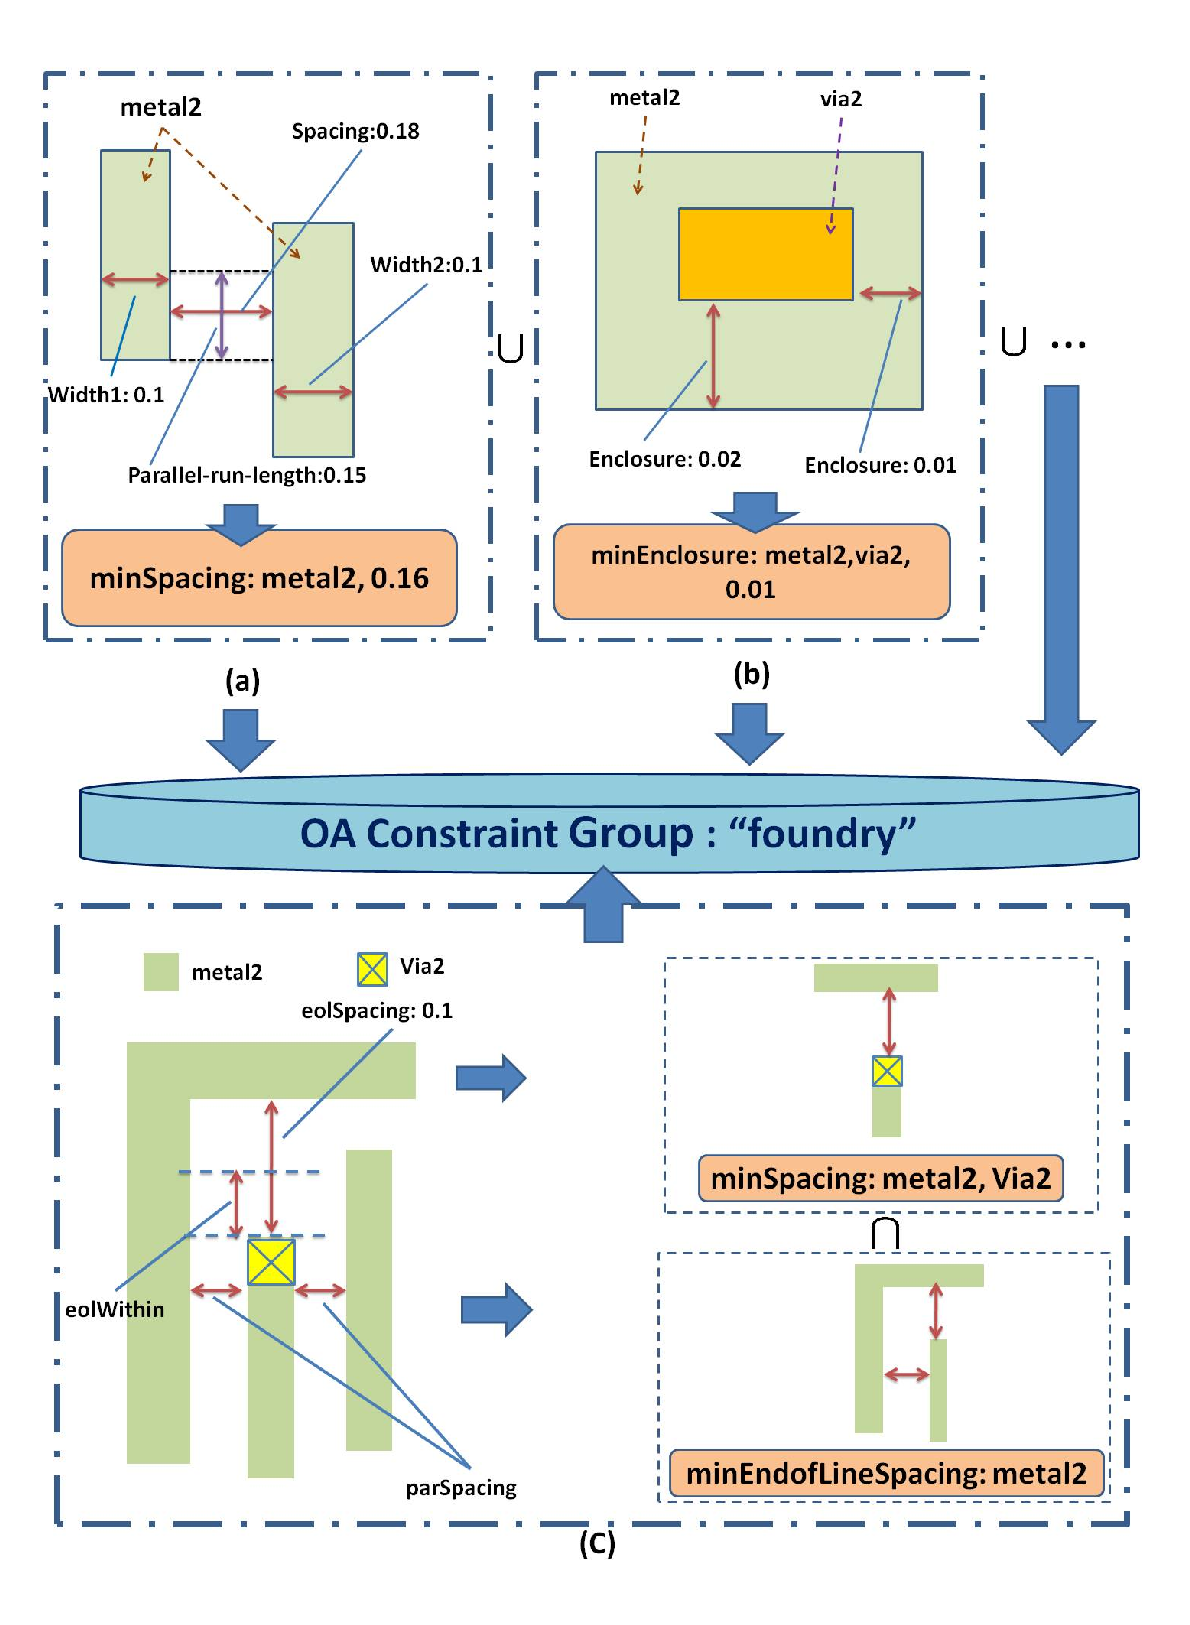
\includegraphics[width=0.5\textwidth]{Fig/Chapter3/SimpleRuleCon2.eps}
        \caption{Mapping simple process rules to constraint group ``foundry''. (a) minimum spacing 0.16um on metal2. (b) minimum enclosure 0.01 with metal2 and via2. (c)Integration of minEndofLineSpacing and minSpacing to fulfill the rule.}
        \label{fig:SimruleCon}
      \end{figure}
    
      Fundamentally, OpenAccess constraint semantic supports basic geometric rules for a single layer or multiple layers. Fig.~\ref{fig:SimruleCon}(a) shows a sample of minimum spacing of two shapes with the same metal, and we can also see minimum enclosure constraint that a layer(via2) is fully enclosed into another layer(metal2) in Fig.~\ref{fig:SimruleCon}(b). It is feasible to transfer these kind of accurate process rules into constraint group.

      However, the basic geometric constraint type no longer satisfied the advanced technology process rule. Many conservative process rules are raised by the foundry due to DFM issues. Fortunately, the OpenAccess constraint group utility supports logical operation among constraints, which means that two or more constraints built-in constraints can form a harder constraint union. In Fig.~\ref{fig:SimruleCon}(c), we can see that a process rule objective is to avoid violation that the minimum spacing between the end of a line from a via on a rectangle-shape metal and its neighbors. By logical interaction of basic physical constraints, minimum spacing to end-of-line (eol) for ``metal2'' and minimum spacing for ``metal2'' and ``via2'', the constraints exactly cover the rule which avoids violation.
      
      By a procedure of operation on transferring the process rules, the built-in constraint group of the foundry can be constructed.

    \subsection{Pre-defined Design Guidelines Constraint Group Generation}\label{sec:PreDesignCG}
    %According to Fig.~\ref{fig:CG}, 
      
      Except the ``foundry'' constraint groups, each design can create their own custom constraint group with arbitrary semantics. Thus, two different circuit designs which share the same technology constraint group tend to preserve totally diversed constraint groups with distinct design purposes. Moreover, even dissimilar objectives are applied on the same analog design with respect to the same technology for particular performance requirement. Thus, the flexibility of user-defined constraint groups is important to have. 

      Traditionally, experienced analog designers manually annotate design constraints on the schematic view. The constraints are mostly related to performance intention, such as symmetrical constraints, proximity group and net ordering. Nevertheless, due to non-unified annotation, the instruction made by the designers cannot be exchanged with a general data model. Here we standardize aforementioned analog constraints into OpenAccess constraint format. 
    
      Other than extracting all the design conditions from an analog layout, we pick only symmetry and proximity constraints to demonstrate of user-defined constraint generation. According to strict hierarchy properties of analog design, if each element in the design has more than 2 constraints, the priority of these constraints is pre-defined by designers knowledge. Therefore, the constraint group can preserve not only the constraint type but also the hierarchical structure. Table~\ref{tableConType} shows the sample constraint type and value which can be preserved in OpenAccess constraint group data model. The constraint definitions below are symmetrical and matching constraints: 


      \newtheorem{Cons}{Constraint}
      \begin{Cons}
        {\bf MatchGroup}, a collection of cells which should be grouped in proximity. It defines the name of MatchGroup, and a series of names of cells.
      \end{Cons}
      \begin{Cons}
        {\bf SymGroup}, a symmetrical pair accompanied with a pre-defined symmetry line by SymLine constraint. The members of symmetrical pair can be cell name or group name defined by MatchGroup or other SymGroup name.
      \end{Cons}
      \begin{Cons}
        {\bf SymLine}, which shows the coordinate type and value of symmetry-axis for layout.
      \end{Cons}
    
    
      \begin{table}[ht]
        \centering
        \caption{Constraint sample type and value for layout design guidelines}\label{tableConType}
        \begin{scriptsize}
          \begin{tabular}[t]{|l|l|}
            \hline
            Constraint Type & Value \\
            \hline
            Symmetry Line & SymLine(name,axis-type,coordinate)  \\
            \hline
            Matching Group  & MatchGroup(name,list-of-cells)  \\
            \hline
            Symmetry Group  & SymGroup(name,Symline,pairs)  \\
            \hline
          \end{tabular}
        \end{scriptsize}
      \end{table}


      \begin{figure}[ht]
        \centering
          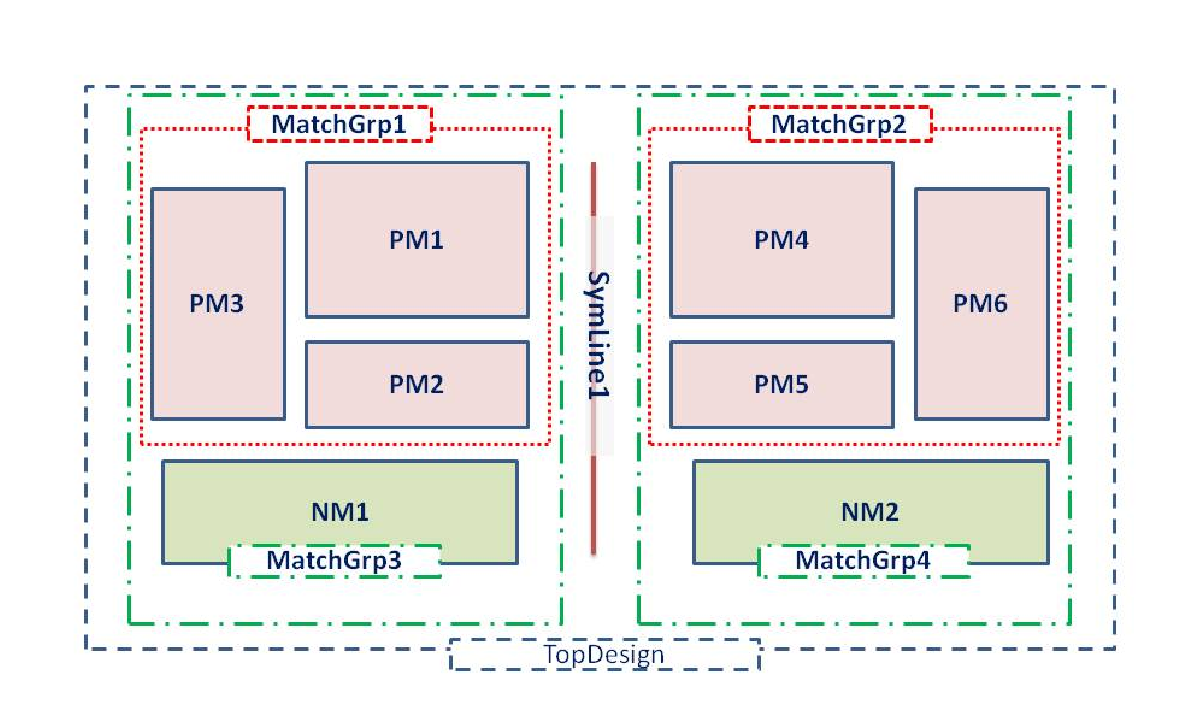
\includegraphics[width=0.7\textwidth]{Fig/Chapter3/PreCG.eps}
        %\begin{spacing}{1}
        \begin{scriptsize}
        \begin{tabular}[t]{l}
          \toprule
        % \hline
          \multicolumn{1}{c}{Constraints in TopDesign}  \\
          \midrule
        % \hline
          SymLine(``SymLine1'',y,0) \\
        % \hline
          MatchGroup(``MatchGrp1'',(``PM1'',``PM2'',``PM3'')) \\
        % \hline
          MatchGroup(``MatchGrp2'',(``PM4'',``PM5'',``PM6'')) \\
        % \hline
          MatchGroup(``MatchGrp3'',(``MatchGrp1'',``NM1'')) \\
        % \hline
          MatchGroup(``MatchGrp4'',(``MatchGrp2'',``NM2'')) \\
        % \hline
          SymGrp(``SymGrp1'',``SymLine1'',(``MatchGrp3'',``MatchGrp4''))  \\
        % \hline
        \bottomrule
        \end{tabular}
        \end{scriptsize}
        %\end{spacing}
        \caption{Pre-defined Constraint Group with layout cell blocks illustration.}
        \label{fig:PreCG}
      \end{figure}
    
    
      We demonstrate the usage of constraint group in Fig.~\ref{fig:PreCG} to annotate design conditions of layout. There are 8 cells including six PMOS and two NMOS in the layout. The pre-defined constraints are illustrated in the table of Fig.~\ref{fig:PreCG} for layout at the top of Fig.~\ref{fig:PreCG}. There are matching group, symmetry group and symmetrical line for symmetry constraint. The priority of constraints is flexible to decide. Here Fig.~\ref{fig:PreCG} shows that matching group has higher ranking in constraint group. For example, PM2 is owned by ``MatchGrp1'' and ``SymGrp1'', but there is only a pair of cells or groups which can be a pair of each symmetry group in this format. We pick PM2 to be a child of  ``MatchGrp1'', then ``MatchGrp1'' is one of a child of ``MatchGrp3''. Therefore, ``MatchGrp3'' is symmetrical to ``MatchGrp4'' by ``SymLine1''. Finally, a group of constraints can exactly cover the symmetry and proximity constraints from design guidelines.


    \subsection{Layout Constraint Extraction}\label{sec:LayoutConExt}
      After extracting constraint rules from the process rules of the foundry, if there are no design guidelines left in the design, we attempt to extract constraints from the existing layout. Without the pre-defined constraint group generated in the previous step, our constraint extraction applies the methodology \cite{srm-massier-tcad08,palpndg-iccad2011}, shown in Fig.~\ref{fig:CGExtract}. Here the extractor complies with the priority that matching constraint is precedential to symmetrical constraint. In the end, the extraction obtains the proximity and symmetry constraints from the layout after placement step. The constraint group generated by the extraction is similar to the pre-defined constraint group represented in Fig.~\ref{fig:PreCG} with the same constraint order. Finally, we integrate these constraints into our hierarchical constraint group for constraint driven routing.
    
      \begin{figure}[ht]
        \centering
        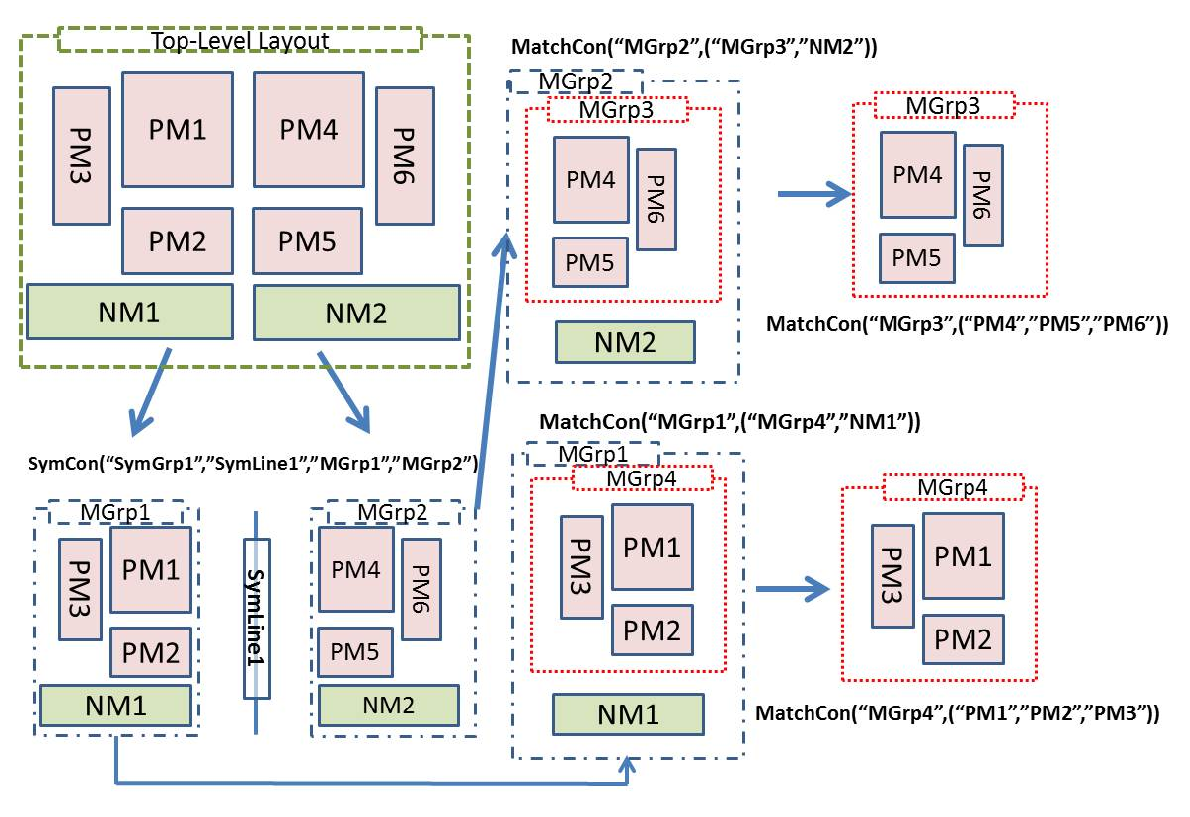
\includegraphics[width=0.7\textwidth]{Fig/Chapter3/CGExtract.eps}
        \caption{Constraints extracted from the existing layout without pre-defined design conditions. The original top-level layout has PM1-PM6 and NM1,NM2. First of all, the top-level layout is divided into a symmetric pair with MGrp1 and MGrp2 via SymLine1. Recursively, MGrp1 and MGrp2 are partitioned in the sub-level. MGrp1 is separated as MGrp3 and NM2, and MGrp2 is separated as MGrp4 and NM1 similarly. In the bottom level, MGrp3 is consisted of PM4-PM6 and MGrp4 is consisted of PM1-PM3}
        \label{fig:CGExtract}
      \end{figure}

  \section{Hierarchical Constraint-Driven Routing}\label{sec:HCDR}

    In this chapter, we introduce a divide-and-conquer approach methodology for analog constraint driven routing as Algorithm~\ref{alg:HCDR} hierarchical constraint driven routing(HCDR) depicts. The basic idea of our methodology is to partition the layout recursively according to constraint group we have generated in previous section. Once the recursion reaches the bottom level of the layout, a priority-free routing for each level of design is applied. We terminate the process when the top level of layout is routed. 

    \subsection{Hierarchical Framework}\label{sec:HierFramework}

      For a hierarchical constraint driven routing (HCDR), an analog layout design accompanied with constraint group is required. The constraint group is generated from the technology process rules and analog design guidelines we have mentioned in Section~\ref{sec:ConGenUni}. First of all, HCDR retrieves constraints one by one from the constraint group. If it is a symmetrical constraint, HCDR splits the symmetry pair and applies sub-level HCDR for them. Similarly, if it is matching constraint, HCDR straightly partitions the existing layout into one matching group and the other. In the end of layout partitioning, we apply a routing-engine in a bottom-up style until the overall layout is fully connected. The common notations used in the rest of this paper are listed in Symbol List.

      \renewcommand{\algorithmicrequire}{\textbf{Input:}}
      \renewcommand{\algorithmicensure}{\textbf{Output:}}
      \renewcommand{\algorithmiccomment}[1]{// #1}
      \newcommand{\HCDR}{\ensuremath{\mbox{\sc HCDR}}}
      \begin{algorithm}[t]
      \caption{$\HCDR(T,CG_T,N)$}\label{alg:HCDR}
      \begin{algorithmic}[1]
      \REQUIRE T: Top-level Design with cells 

      $CG_T$: Constraint-group of the top-level design.

      N: a list of nets w.r.t. the top-level design.
      \ENSURE $T^r$ : Top-level design after routing.
      \medskip

      \WHILE {$num(CG_T) \geq 1$}
        \STATE $Con \gets pop(CG_T) $
        \IF{$Con \in SymCon$}   
          \STATE $(SymGrp,T') \gets partition(T,Con)$
          \STATE $({SymGrp}_L,CG_L) \gets getLeft(SymGrp,Con,CG_T)$
          \STATE $({SymGrp}_R,CG_R) \gets getRight(SymGrp,Con,CG_T)$
          \STATE ${CG}_L \gets getCG({SymGrp}_L,Con,CG_T)$
          \STATE ${CG}_R \gets getCG({SymGrp}_R,Con,CG_T)$
          \STATE $T^r \gets merge(T^r,\HCDR({SymGrp}_L,CG_L,N))$
          \STATE $T^r \gets merge(T^r,\HCDR({SymGrp}_R,CG_R,N))$
          \STATE $T = T'$
        \ELSIF {$CG \in MatchCon$}      
          \STATE $(MatchGrp,CG_M,T') \gets partition(T,Con)$
          \STATE $CG_M \gets getCG(MatchGrp,Con,CG_T)$
          \STATE $T^r \gets merge(T^r,HCDR(MatchGrp,CG,N))$
          \STATE $T = T'$
        \ENDIF
      \ENDWHILE
      \STATE $T^r \gets merge(T^r,T)$
      \STATE $T^r \gets route(T^r,CG_T,N)$
      \RETURN $T^r$ \COMMENT{Terminate when $T^r$ is routed}
      \end{algorithmic}
      \end{algorithm}

      %\begin{table}[ht]
      %  \centering
      %  \caption{Notations used in HCDR}\label{tableNotation}
      %  \begin{scriptsize}
      %  \begin{tabular}[t]{|l|l|}
      %    \hline
      %    $T$       & Top-level Design with cell blocks \\
      %    \hline
      %    $T'$      &   design T after partition      \\
      %    \hline
      %    $T^r$       &   T with partial routing completed  \\
      %    \hline
      %    $CG_T$      & Constraint group of the current level design  \\
      %    \hline
      %    $N$       & list of connectivity w.r.t. the design T  \\
      %    \hline
      %    $Con  $   & constraint pop out from $CG_T$    \\
      %    \hline
      %    $SymCon$    & symmetrical constraint in $CG_T$  \\
      %    \hline
      %    $MatchCon$    & matching constraint in $CG_T$   \\
      %    \hline
      %    $getCG$     & obtaining constraint group for partitioned design \\
      %    \hline
      %    $SymGrp$    & symmetrical group described in SymCon \\
      %    \hline
      %    $MatchGrp$    & matching group described in MatchCon  \\
      %    \hline
      %    $num(CG_T)$   & total number of constraints in $CG_T$ \\
      %    \hline
      %  \end{tabular}
      %  \end{scriptsize}
      %\end{table}


    \subsection{Symmetrical and Matching Group Partition}\label{sec:SMGrp}
      
      If HCDR encounters a symmetry constraint, the current design should be partitioned into two parts, which are the symmetrical group and another group. The symmetrical group consists of the left group $SymGrp_L $ and the right group $SymGrp_R$. Also, the constraint group for left and right groups are extracted from the current top-level constraint group. We continue to perform HCDR recursively for both of them. Since the HCDR returns a routed layout after termination, we then merge the symmetry pair into $T^r$. Each part of $T_r$ is routed, and the final merge will be performed. 

      When the popped constraint is matching constraint, similar to symmetrical group division, HCDR tends to distribute the existing layout according to the matching constraints. In each iteration, HCDR splits a MatchGrp from the layout and then performs the next level HCDR of such sub-design. After a routed design is returned from the child's HCDR, it is merged into $T_r$. Until all the symmetric and matching groups are completed, the rest parts of the design are routed.

    \subsection{Bottom-up Routing}\label{sec:HCDR_BtmUp}

      When there is no constraint left in the constraint group for partitioning, we apply a merge routing mechanism to connect all the nets in the current level of HCDR. Since the routing algorithm is applied in hierarchical way, HCDR only deal with the connectivity between the cells in the current level. In case of routing between two groups, such as one $SymGrp_L$ and another $SymGrp_R$, the routing is utilized for the inter-pins among groups. The intra-pin routing is completed by the lower level HCDR. Since the routing order is decided by the constraint group generation step, it is possible to cause violation after merging into $T_r$. For the sake of avoiding to overlap with other group of layout, the routing region of the current level HCDR is fixed to the contour outside the blocks. 

      In summary, HCDR performs a divide-and-conquer approach for hierarchical routing w.r.t. the routing order which is determined in the constraint group. However, A net with mutiple pins in different constraint groups are routed with trivial detour. Even though divide-and-conquer approach for routing lose optimal wirelength due to the hierarchical structure, the process variation issue will be reduced by following critical analog constraints at routing stage. Additionally, Since the constraint group can be preserved before the routing stage, it is configurable that HCDR is able to generate different routing results by manipulating the structure of such constraint group. This paper illustrates the comparison in Section~\ref{sec:CUCLMExp}. The top-down flow divides the layout design and the bottom-up flow routes the design by each level. Note that, if the constraint group is defined in another kind of grouping order for the layout, the routing result will be different.
  
  \section{Experimenta Results}\label{sec:CUCLMExp}

    \begin{sidewaystable}[ht]
      %\definecolor{mygray}{gray}{.9}

      \caption{Routing statistics and performance comparison on analog high-speed output interface with pre-simulation, manual-route, flatten-route, HCDR-LE and HCDR-PD routing methodology.}
      \label{table:HCDRResult}
      \begin{lrbox}{\tablebox}
      \begin{threeparttable}
      \begin{small}
      \begin{tabular}{|l|c|c|c|c|c|c|c|c|c|c|c|c|c|c|}
            \hline
                    & \multicolumn{4}{c|}{Routing result} & \multicolumn{5}{c|}{3GHz frequency simulation} 
                       & \multicolumn{5}{c|}{4GHz frequency simulation}\\ \cline{2-15}
            Circuit     & wirelength  & Via\#   & runtime & DRC     & Eye Height  &P-to-P     & RMS     &Rise Slope 
            & Fall Slope  & Eye Height  &P-to-P   & RMS   &Rise Slope & Fall Slope\\
                    & (${\mu}m$)  &     &     & errors  & (mV)    & Jitter(ps)  & Jitter(ps)&(mV/ps)          
            & (mV/ps)   & (mV)    &Jitter(ps) & Jitter(ps)&(mV/ps)  & (mV/ps) \\  
            \rowcolor{black}
            \hline
            \rowcolor{mygray}
            pre-sim         & -     & -   & -     & -   & 297     & 6.54    & 1.08    & 6.14    
            & -8.5    & 290     & 7.01  & 1.7   & 5.69  & -8.65 \\    
            \hline
            manual-route\tnote{a} & 617.845   &   32    & 1 week    & 0   &{\bf 337.6}  & 6.81    & 1.46    & 4.61    
            & -7.22   & 302     & 9.29  & 1.67    & 4.67  & -6.52 \\
            \hline
            flatten-route\tnote{b}  & {\bf 497.58}& 251   & 192sec.   & 106   & 292.8   & 6.82    & 1.33    & 4.93    
            & -7.96   & 276     & 9.83  & 1.78    & 5.29  & -7.29 \\
            \hline
            HCDR-LE\tnote{c}    &   632     &{\bf 238}  &{\bf121sec.} & 11    &   334     & 6.47    &{\bf 1.24} &{\bf 6.87} 
            & -7.98   & 278.8   & 8.55  & 1.61    & 4.03  & -8.97 \\
            \hline
            HCDR-PD\tnote{d}    &   611.005   & 285   & 149sec.   & {\bf7}  & 310     &{\bf 6.23} & 1.26    & 5.46    
            &{\bf -8.28}  & {\bf 327} &{\bf 8.52} &{\bf 1.52} & {\bf 5.57}  &{\bf -9.01}\\  
            \hline
      \end{tabular}
      \end{small}
      \begin{tablenotes}
        \item [a] a routing result done by analog layout designer manually.
        \item [b] a routing result done by an industrial router without hierarchical constraints.
        \item [c] HCDR with constraint group extracted from layout as matching-first-symmetrical-last order.
        \item [d] HCDR with pre-defined constraint group from designers as symmetrical-first-matching-last order.
      \end{tablenotes}
      \end{threeparttable}
      \end{lrbox}
      \scalebox{0.8}{\usebox{\tablebox}}
    \end{sidewaystable}


    In this section, we present and compare the experimental results among:
    \begin{enumerate}
      \item {\bf Manual routing,} the layout is completed by manual routing.
      \item {\bf Flatten-routing,} which performs only maze-route and  
      \item {\bf HCDR-PD}, it performs HCDR with symmetric first constraints which are predefined by design knowledge. 
      \item {\bf HCDR-LE}, it performs HCDR with matching first constrains which are extracted from post-placement layout.
    \end{enumerate} 
    Our methodologies were implemented in C++ language with OpenAccess library version 2.2.04p54. We compile and execute our program on a workstation with AMD Phenom(tm) II X4 925 2.8GHz processor and 8GB memory under the Red Hat 4.6 Linux operation system. We apply an maze-route-style industrial engine in the bottom level routing which can considering the foundry level constraint simultaneously. We compare our methodology with high speed I/O interface of one industrial SoC chip design. Such SoC design includes a digital functional block, a clock-tree network and one analog block. There are 378 n-type and 362 p-type mosfets in this analog design with area 15.8x68.37 ${{\mu}m}^2$. This design is working on 40nm technology for supply voltage 1.1V. Since the design is confidential, we only show the routing information and post-layout simulation result for comparison.

    As there is no previous work that handles analog routing based on constraint driven hierarchical module, we compare the performance by HSPICE simulation among schematic and the routing results. Moreover, to practice the functionally of our configurable constraint group, we provide the routing result with two compisitions of constraints, HCDR-PD and HCDR-LE. For our HSPICE simulation, we practice on two kinds of frequency with 3GHz and 4GHz. For the performance comparison, we first compare the design performance specification illustrated in Table \ref{table:HCDRResult}. Since the functionality of the analog block is the output stage of the digital block in the SoC chip, we tend to analyze the performance difference with {\bf Eye Diagram} of the output waveform for signal integrity. According to the measurements in~\cite{eyediagram}, the following parameters should be measured: {\bf Eye Height}, {\bf Peak-to-Peak(P-2-P) Jitter}, {\bf RMS Jitter}, {\bf Rise Slope} and {\bf Fall Slope} in the eye diagram of each pattern. For routing comparison, although flatten-routing obtained better wirelength than other routing methods, it violates process rule severely by DRC checking. 
    
    Furthermore, HCDR interacts with foundry constraint group well much fewer DRC errors. From this results, we can tell that the integrated foundry-intension constraints efficiently deals with advanced technology rules. In 3GHz simulation, other than manual-route, HCDR-LE achieves 13\%, 12.4\% and 7.7\% improvement for eye-height over flatten-route, pre-sim and HCDR-PD, respectively. Since eye-height represents the impact from signal-to-noise, the larger eye height(open-eye), the better signal integrity with voltage amplitude. RMS jitter and P-to-P jitter are required to be measured for jitter characterization. As expected, HCDR-LE have achieved remarkable success in RMS jitter. Additionally, HCDR-PD obtains P-to-P jitter reductions of 0.31ps, 0.58ps, 0.59ps and 0.24ps over pre-sim, manual-route, flatten-route and HCDR-LE, respectively. Since pre-defined constraint group for HCDR-PD honors the symmetrical constraint than matching constraint, we can tell that the matching net of symmetrical constraint guarantees lower variation. 
  
  
    \begin{figure}[ht]
      \centering
      \begin{subfigure}[t]{0.4\textwidth}
        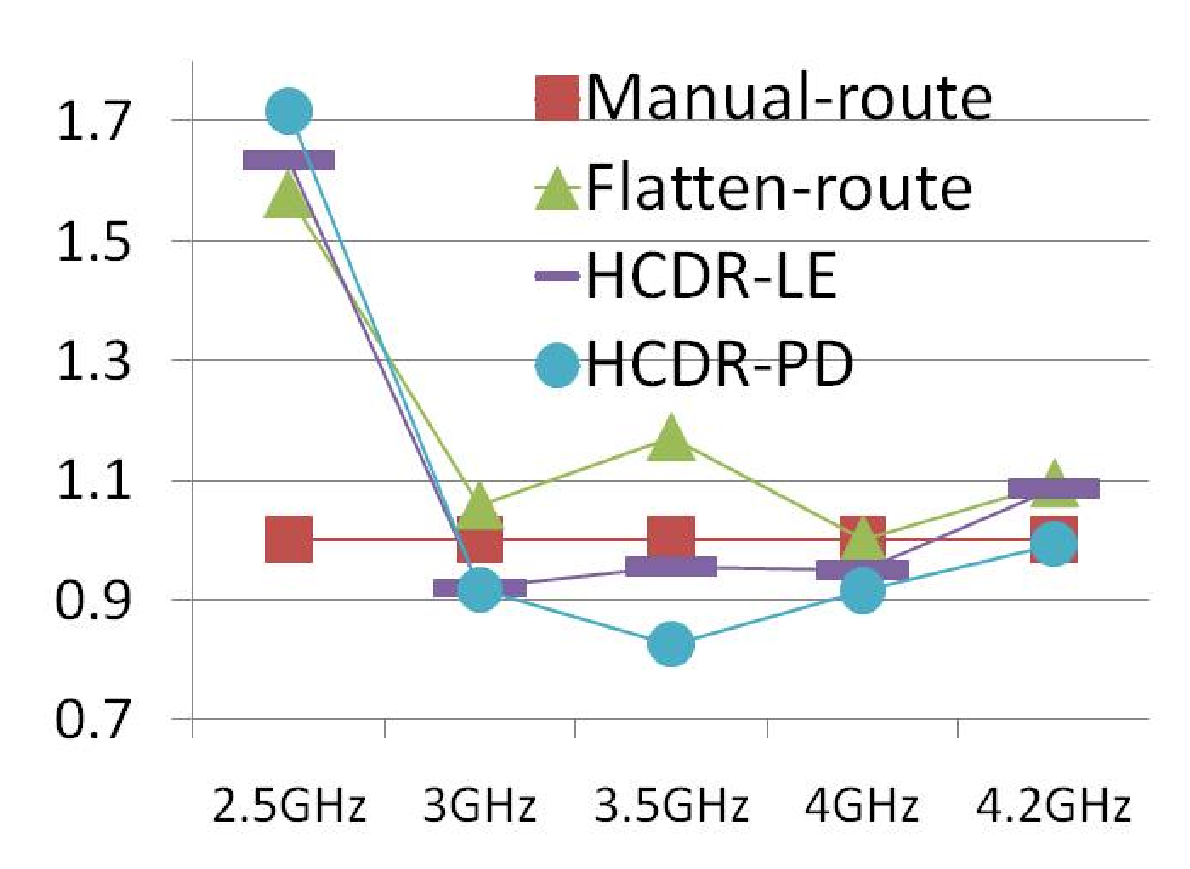
\includegraphics[width=\textwidth]{Fig/Chapter3/P2PJitter.eps}
      \caption{P2P Jitter}\label{P2PJitter}
      \end{subfigure}
      \begin{subfigure}[t]{0.4\textwidth}
        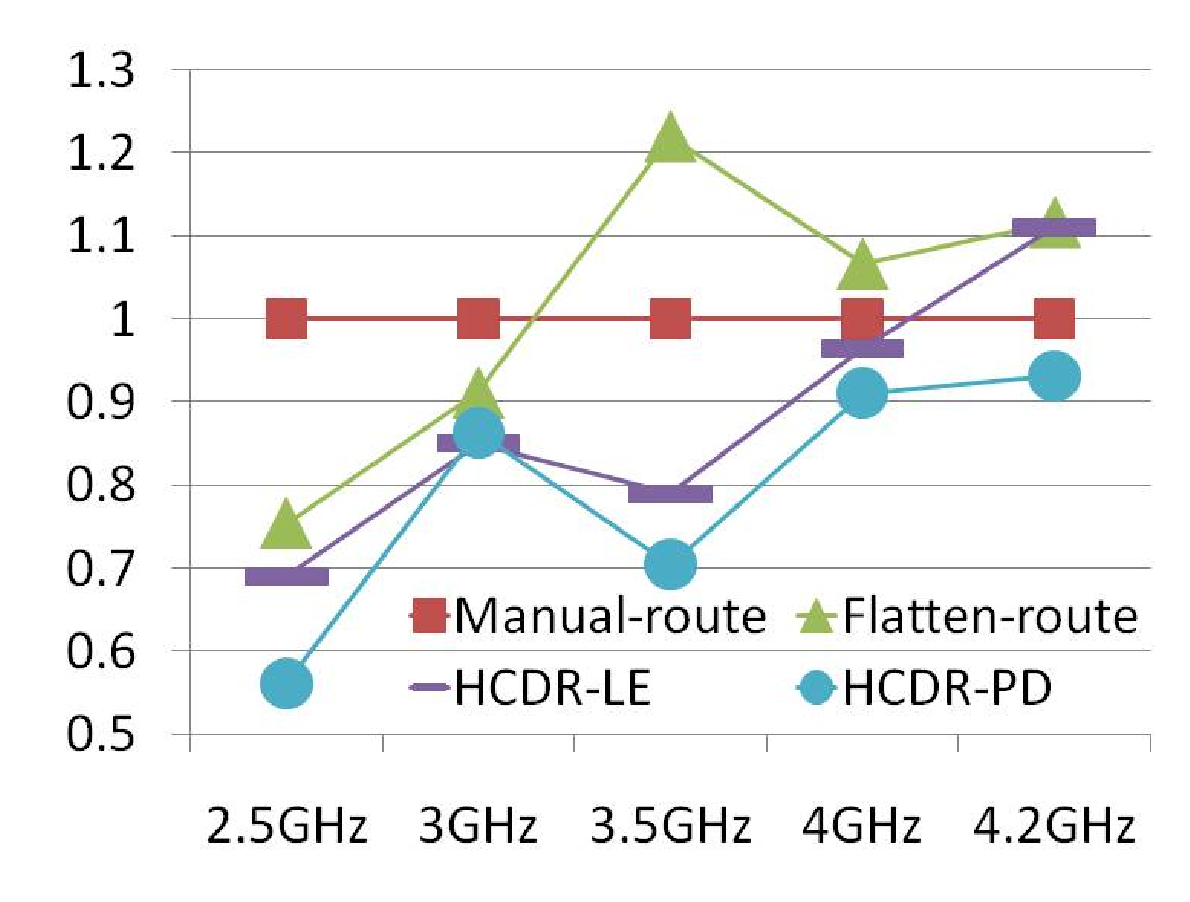
\includegraphics[width=\textwidth]{Fig/Chapter3/RMSJitter.eps}
        \caption{RMS Jitter}\label{RMSJitter}
      \end{subfigure}
      \caption{Normalized(by manual-route) jitter characteristics with different frequencies for manual-route, flatten-route, HCDR-LE and HCDR-PD.}\label{fig:Jitter}
    \end{figure}
    
    We also receive better rising time and falling time by HCDR-LE and HCDR-PD. In this case, HCDR-LE achieves 11.9\%, 50\%, 40\% and 25\% improvement over pre-sim, manual-route, flatten-route and HCDR-PD respectively. On the other hand, HCDR-PD also shows 14.7\%, 4\% and 3.8\% better performance with fall slope over manual-route, flatten-route and HCDR-LE results respectively. Moreover, for higher frequency as 4GHz, HCDR-PD achieves better performance on P-to-P jitter, RMS jitter and rise slop of eye diagram than flatten-route and HCDR-LE. It is obvious that our HCDR-PD performs better on signal transition in eye hight and fall slope to the others. 
    
    Further signal jitter characteristics among routing results are shown in Fig.~\ref{fig:Jitter}. In Fig.~\ref{P2PJitter}, we see HCDR-PD obtains better in higher frequency. In addition, HCDR-PD maintains performance over other routing results by RMS jitter, shown in Fig.~\ref{RMSJitter}. Since HCDR-PD honors the symmetrical constraint with higher priority, the routing result retrieves much stronger signal integrity with noise shielding and crossing variation than the flatten-route for all and manual-route in most cases. It is clear that our HCDR methodology can provide a better solution for routing order which is defined by constraint group. Our layout constraint extractor generates and performs routing order according to placement topology in success. Furthermore, we can see that the HCDR-PD, which preserves the design guidelines by constraint group, can obtain routing result with pre-defined constraint.

  \section{Summary}\label{sec:CUCLMSum}

    In this chapter, we generate the uniform constraint format for analog constraint driven routing. We have proposed hierarchical constraint driven routing mechanism that is faithful to the constraint group we have generated. HCDR reconfigures the analog routing order according to constraints, then the bottom-up routing is applied with respect to the order of constraints. In addition to handling technology process rule, we not only generate the constraint from existing layout topology after placement, but also preserve the design guidelines by experienced designers for analog routing purpose. The methodology can be used to generate routing automatically with different combinations of constraint group. The future work will mainly focus on the extension of the configurable analog constraints like electromagnetic effect, and on the symbolic routing which adopting this configurable analog constraints with better performance

